\documentclass[12pt, onecolumn, oneside]{gsajnl}

\articletype{gs} % article type

\usepackage{setspace}
\usepackage{lineno}
\usepackage{pdflscape}
\usepackage{xr}
\usepackage{enumitem}
\usepackage[export]{adjustbox}
%\usepackage{xr}
%\externaldocument{supplemental/odds_ratio_transformation_supp}
\usepackage{subfig}


%--------------------------------------------------------------------------------------------------------------------------%
%--------------------------------------- New commands ------------------------------------------------------------%

%\newcommand{\beps}{\bar{\epsilon}}
\newcommand{\balg}{\begin{alg}}
\newcommand{\ealg}{\end{alg}}
\newcommand{\ceil}[1]{\left\lceil #1 \right\rceil}
\newcommand{\floor}[1]{\left\lfloor #1 \right\rfloor}
\newcommand{\Shan}{{\EuScript{H}}}
\newcommand{\KL}{{\EuScript{D}}}
\newcommand{\El}{{\EuScript{E}}}
\newcommand{\MI}{\EuScript{M}} % mutual information
\usepackage[labelsep=space,labelfont=bf]{caption}
%\newcommand{\Fish}{\EuScript{I}}
\newcommand{\bvo}{\mbox{$\bv_{0}$}}
\newcommand{\bS}{\mathbf{S}}         
\newcommand{\bL}{\mathbf{L}}                            
\newcommand{\bs}{\mathbf{s}}
\newcommand{\bQ}{\mathbf{Q}}
\newcommand{\bG}{\mathbf{G}}
\newcommand{\bg}{\mathbf{g}}
\newcommand{\bincof}[2]{{{#1} \choose {#2}}} 
\newcommand{\gr}{\mbox{$\nabla$}}

\renewcommand{\figurename}{{\bf{Fig.}}}                                        % Figure name
\newcommand{\eps}{\epsilon}                                                          % Epsilon
\newcommand{\beps}{{\boldsymbol \epsilon}}                                 % Bold Epsilon
\newcommand{\st}{\: : \:}                                                                  % Such that
\newcommand{\Lh}{\EuScript{L}}                                                     % Likelihood
\newcommand{\Sc}{\EuScript{S}}                                                     % Score function
\newcommand{\bigO}{\EuScript{O}}                                                 % Big O notation
\newcommand{\lito}{$o$}                                                                  % Little o notation
\newcommand{\bl}{\mbox{\boldmath $\ell$}}                                    % Log likelihood                               
\newcommand{\bSigma}{\mbox{\boldmath $\Sigma$}}                    % Bold big sigma
\newcommand{\bsigma}{\mbox{\boldmath $\sigma$}}                    % Bold big sigma
\newcommand{\bB}{\mathbf{B}}                                                       % Bold big B
\newcommand{\bb}{\mathbf{b}}                                                       % Bold little b
\newcommand{\bz}{\mathbf{z}}                                                        % Bold z
\newcommand{\bX}{\mathbf{X}}                                                       % Bold big X
\newcommand{\bx}{\mathbf{x}}                                                        % Bold little x
\newcommand{\bbeta}{{\boldsymbol \beta}}                                     % Bold beta
\newcommand{\bhbeta}{\hat{\bbeta}}                                              % Bold beta hat

\newcommand{\bk}{\mathbf{k}}
\newcommand{\bq}{\mathbf{q}}
\newcommand{\be}{\mathbf{e}}
\newcommand{\bF}{\mathbf{F}}
\newcommand{\bK}{\mathbf{K}}
\newcommand{\br}{\mathbf{r}}
\newcommand{\by}{\mathbf{y}}
\newcommand{\bZ}{\mathbf{Z}}
\newcommand{\bu}{\mathbf{u}}
\newcommand{\bU}{\mathbf{U}}
\newcommand{\bY}{\mathbf{Y}}
\newcommand{\bP}{\mathbf{P}}
\newcommand{\bR}{\mathbf{R}}
\newcommand{\bV}{\mathbf{V}}
\newcommand{\bW}{\mathbf{W}}
\newcommand{\bT}{\mathbf{T}}
\newcommand{\bt}{\mathbf{t}}
\newcommand{\dotsim}{\stackrel{\centerdot}{\sim}}
\newcommand{\bnu}{\vect{\nu}}
\newcommand{\btheta}{\vect{\theta}}
\newcommand{\blambda}{\vect{\lambda}}
\newcommand{\halmos}{\vspace{3mm} \hfill \mbox{$\Box$}}
\newcommand{\bE}{\mathbf{E}}
%\newcommand{\bJ}{\mbox{\boldmath $J$}}
\newcommand{\ba}{\mathbf{a}}
\newcommand{\bh}{\mathbf{h}}
\newcommand{\bfb}{\mathbf{b}}
\newcommand{\bff}{\mathbf{f}}
\newcommand{\bA}{\mathbf{A}}
\newcommand{\bM}{\mathbf{M}}
\newcommand{\bN}{\mathbf{N}}
\newcommand{\bc}{\mathbf{c}}
%\newcommand{\bc}{\begin{center}}
\newcommand{\bbf}{\mathbf{f}}
%\newcommand{\bd}{\mathbf{d}}
\newcommand{\bw}{\mathbf{w}}
\newcommand{\bsb}{\boldsymbol \beta}
\newcommand{\SCV}{\text{SCV}}
\newcommand{\cov}{\text{Cov}}
\newcommand{\Supp}{\text{Supp}}
\newcommand{\bp}{\mathbf{p}}
\newcommand{\bC}{\mathbf{C}}
\newcommand{\bii}{\mathbf{i}}
\newcommand{\bjj}{\mathbf{j}}
\newcommand{\bII}{\mathbf{I}}
\newcommand{\bv}{\mathbf{v}}
\renewcommand{\epsilon}{\varepsilon}
\renewcommand{\rho}{\varrho}
%\renewcommand{\log}{\ln}
\renewcommand{\hat}{\widehat}
\renewcommand{\tilde}{\widetilde}
\renewcommand{\leq}{\leqslant}
\renewcommand{\geq}{\geqslant}
\newcommand{\argmax}{\mathop{\rm argmax}}
\newcommand{\argmin}{\mathop{\rm argmin}}
\newcommand{\iid}{\text{iid }}
\newcommand{\elite}{\mathop{\rm e}}
\newcommand{\obs}{\mathop{\rm obs}}
\newcommand{\mis}{\mathop{\rm mis}}
\newcommand{\fin}{\mathop{\rm fin}}
\newcommand{\start}{\mathop{\rm start}}
\newcommand{\tot}{\mathop{\rm tot}}
\newcommand{\difr}{\mathop{\rm difr}}
\newcommand{\Conv}{\mathop{\mathbf{Conv}}}
\newcommand{\Ber}{{\sf Ber}}
\newcommand{\ber}{{\sf Ber}}
\newcommand{\Dir}{{\sf Dir}}
\newcommand{\Erl}{{\sf Erl}}
\newcommand{\bin}{{\sf Bin}}
\newcommand{\Weib}{{\sf Weib}}
\newcommand{\Cauchy}{{\sf Cauchy}}
\newcommand{\negbin}{{\sf NegBin}}
\newcommand{\mnom}{{\sf Mnom}}
\newcommand{\Geom}{{\sf Geom}}
\newcommand{\NE}{{\sf NE}}
\newcommand{\Hyp}{{\sf Hyp}}
\newcommand{\Poi}{{\sf Poi}}
\newcommand{\Po}{{\Poi}}
\newcommand{\U}{{\sf U}}
\newcommand{\ex}{{\sf Exp}}
\newcommand{\Nor}{{\sf N}}
\newcommand{\pareto}{{\sf Pareto}} % pareto
\newcommand{\gam}{{\sf Gamma}}
\newcommand{\bet}{{\sf Beta}}
\newcommand{\weib}{{\sf Weib}}
\newcommand{\DU}{{\sf DU}}
\newcommand{\SE}{{\sf SExp}} % shifted exponential
\newcommand{\DE}{{\sf DExp}} % double exponential
\newcommand{\nbin}{{\sf NBin}}
\newcommand{\Em}{\mathbb E}
\newcommand{\Pm}{\mathbb P}
\newcommand{\R}{\mathbb R}
\newcommand{\B}{{\cal B}}
\newcommand{\N}{\mathbb N}
\newcommand{\Z}{\mathbb Z}
\newcommand{\Q}{\mathbb Q}
\newcommand{\C}{\mathbb C}
\newcommand{\bD}{\bf D}
\newcommand{\scA}{\mathscr{A}}
\newcommand{\scB}{\mathscr{B}}
\newcommand{\scC}{\mathscr{C}}
\newcommand{\scF}{\mathscr{F}}
\newcommand{\scI}{\mathscr{I}}
\newcommand{\scJ}{\mathscr{J}}
\newcommand{\scL}{\mathscr{L}}
\newcommand{\scM}{\mathscr{M}}
\newcommand{\scP}{\mathscr{P}}
\newcommand{\scS}{\mathscr{S}}
\newcommand{\scR}{\mathscr{R}}
\newcommand{\scU}{\mathscr{U}}
\newcommand{\scE}{\mathscr{E}}
\newcommand{\scT}{\mathscr{T}}
\newcommand{\scV}{\mathscr{V}}
\newcommand{\scX}{\mathscr{X}}
\newcommand{\scY}{\mathscr{Y}}
\newcommand{\scZ}{\mathscr{Z}}
\newcommand{\gvn}{\,|\,}
\newcommand{\e}{\text{e}}
\newcommand{\Var}{\text{Var}}
\newcommand{\var}{\text{Var}}
\newcommand{\ds}{\displaystyle}
\newcommand{\vect}[1]{\boldsymbol #1}
\newcommand{\vv}[1]{\boldsymbol #1}
\newcommand{\intrusion}[1]{\begin{list}{}%
{\leftmargin\parindent\rightmargin0pt\listparindent0pt\parsep1ex%
\labelwidth0pt\labelsep0pt}\item[]\small\sf$\spadesuit$~#1 \end{list}}
\newcommand{\convdistr}{\stackrel{\cal D}{\rightarrow}}
\newcommand{\di}{\text{d}}
\newcommand{\tr}{\text{tr}}
\newcommand{\n}{\newline}
\newcommand{\cF}{{{\cal F}}}
\newcommand{\cG}{{{\cal G}}}
\newcommand{\cH}{{\cal H}}
\newcommand{\Prob}{\Pm}
%\newcommand{\cas}{{\stackrel{\text{a.s.}}{\longrightarrow}}}
\newcommand{\cas}{\rightarrow}
\newcommand{\ra}{\rightarrow}
\newcommand{\lra}{\leftrightarrow}
\newcommand{\rar}{\rightarrow}
\newcommand{\Rar}{\Rightarrow}
\newcommand{\dar}{\downarrow}
\newcommand{\chg}{\marginpar{*}}
\newcommand{\Ito}{It\^{o}}
\newcommand{\bss}{\boldsymbol}



% ======================================================================================================
% Title page
% ======================================================================================================

%\title{Interpretable effects from disease trait linear mixed model association studies}
\title{The quantification of DNA motifs within flanking sequences of gene expression quantitative trait loci in humans}

% Authors
% ----------

\author[1]{Jacqueline Kiewa}
\author[1]{Loic Yengo}
\author[1]{Luke Lloyd-Jones}


% Affiliations
% -------------

\affil[1]{Institute for Molecular Bioscience, University of Queensland, Brisbane, Queensland 4072, Australia}

\keywords{DNA motifs; Genome-wide association studies; Expression quantitative trait loci}

\runningtitle{DNA motifs} % For use in the footer 
\correspondingauthor{Lloyd-Jones}

%% ======================================================================================================
%% Abstract
%% ======================================================================================================
%
\begin{abstract}
The aim of this research is to identify and quantify DNA sequence motifs that occur within the flanking sequences of gene expression quantitative trait loci (eQTL), which have been derived from genome-wide association analyses of gene transcript abundance in whole blood. It is hypothesised that eQTL influence their targeted gene through regulation, and that the quantification and characterisation of sequence motifs that are enriched in the flanking regions of eQTL will contribute to an understanding of the mechanics and both genomic and individual variation of this regulation. Sequence motifs are short, recurring patterns in DNA that are presumed to have biologically active functions. A subset of the motifs identified through this research may be transcription factor binding sites, which regulate gene expression through enhancing or restricting transcription.
\end{abstract}

\begin{document}
\doublespacing
\maketitle

%--------------------------------------------------------------------------------------------------------------------------%
%--------------------------------------- Begin Document -----------------------------------------------------------%


%--------------------------------------------------------------------------------------------------------------------------%
%--------------------------------------- Introduction-------------------------------------------------------------------%
\clearpage
\section{Introduction}

An important complex trait that differs amongst individuals is the level of gene expression, obtained by measuring the amount of mRNA present in specific tissues. The class of variants that influence this trait has been labelled expression quantitative trait loci (eQTL). These variants are particularly important to GWA studies, since they can help to prioritize likely causal variants amongst the SNPs identified by the GWA study, as well as provide some insight into the biological mechanisms used by organisms to influence complex traits and diseases \citep{albert2015role}. \citet{albert2015role} note that the majority of QTL identified by human GWA studies occur in non-coding regions that are not in LD with coding exons. It is therefore hypothesised that these QTL influence their targeted gene through regulation of its expression \citep{nica2013expression}. A further hypothesis is that an eQTL and its surrounding region will be enriched in biologically active DNA sequence motifs which will contribute in some way to gene expression regulation. 

\citet{lloyd2017genetic} conducted an analysis using data from the Consortium for the Architecture of Gene Expression (CAGE), which comprises individual-level whole-blood expression and genotype data on 2,765 individuals. This analysis identified 11,204  independent cis expression quantitative trait loci (eQTL). The aim of the research is to identify DNA motifs in the genomic regions surrounding the set of cis eQTL identified by \citet{lloyd2017genetic}, following the hypothesis that flanking sequences of an eQTL will be enriched in recurring motifs of DNA that have a biological function, most likely involved in transcription.

DNA sequence motifs are short, recurring sequences in DNA that are thought to have some biological function \citep{d2006dna}. They may form binding sites for proteins such as transcription factors or nucleases, or they may provide signals for important regulatory processes such as methylation, or ribosome binding or mRNA processing \citep{d2006dna}. Gene regulation is an important aspect of the eukaryotic genotype \citep{beckerman2005gene}, changes in which are responsible for much of the phenotypic divergence between and within species \citep{stewart2012transcription}. However, an understanding of the biological mechanisms by which this diversity regulates gene expression has been challenging  \citep{pai2015genetic, gaffney2013global}. Transcription constitutes the first and one of the most intensely regulated steps of gene expression \citep{zabidi2016regulatory}, and a subset of DNA motifs in the region of eQTL are sequence binding sites for transcription factors (TFs). Much research has therefore focused on the identification of transcription factors (TFs) that coincide with eQTL and are likely to enhance or restrict gene expression. However, it has
been hypothesised that altered binding sites are often not associated with any change in gene expression.  Transcription factors frequently bind to each other to form a complex, so that the DNA binding site may be only for the basal transcription factor, with other TF's bound to each other rather than to the DNA. Altered binding sites are often not associated with any change in gene expression.


Once chromatin has become accessible, transcription can initiate within the core promoter site, which recruits RNA polymerase II and assembles the pre-initiation complex \citep{zabidi2016regulatory}. However, transcription will proceed at a very low basal level without the contribution of enhancers. Enhancers are DNA elements up to several hundred bp in length, and contain many short TF binding sites. Either individual or cooperative combinations of TFs are recruited to these sites and function as activators or repressors that regulate transcription from the target core promoter. Despite the abundance of research that has focussed on the relationship between eQTL and transcription factors, as a subset of DNA sequence motifs, TFs form just one piece in the complex jigsaw of gene regulation, with other regulatory processes also playing a part. A de novo motif search by \citet{schor2017promoter}, for example, found a number of core motifs (not TF binding sites) that controlled
the shape of promoter regions, resulting in changed transcription levels. Other systems of gene regulation include methylation of CpG sites, alternative splicing, and post-transcriptional effects such as interaction with miRNAs and polyadenylation \citep{gaffney2013global}. \citet{gaffney2013global} also observed that eQTL are often enriched in exons, and \citet{kirsten2015dissecting}, found that eQTL also coincide with non-coding RNAs and pseudogenes. 
The following overview of potentially important motifs in DNA follows \citep{boeva2016analysis}. Tandem repeats are repeated DNA sequence ordered in a head-to-tail fashion and include microsatellites, minisatellites, and satellite sequences. Short tandem repeats may serve as binding sites for specific transcription factors, whilst longer satellite repeats can influence the 3D structure shaping of the genome. Interspersed repeats are similar sequences to
STRs and are located throughout the genome and include transposable elements such as SINEs and LINEs. AT-rich sequence are often located in gene promoters and play a role in transcription initiation. Approximately 24\% of human genes contain an AT-rich sequence within the core promoter, with 10\% containing a canonical TATA-box motif (TATAWAWR; W = A/T, R = A/G). In general, AT-rich DNA is easier to unwind than GC-rich DNA, since AT base pairing contains fewer bonds than GC base pairs, but this process is amplified by TATA binding protein which is recruited by the TATA-box. GC-rich sequences: The remaining 76\% of human promoters that are GC-rich contain multiple binding sites of the transcriptional activator SP1 \citep{yang2007prevalence}. As much as 56\% of human genes, including most housekeeping genes, possess CpG islands, i.e. 300-3000 bp GC-rich sequences around gene transcription start sites (TSS's) with a high density of GpG dinucleotides. CpG islands have a high methylation level, which is associated with transcriptional repression. Splice sites are involved post initial transcription, when the RNA undergoes the process of splicing, during which introns are removed and the remaining exons are joined together. Generally this process is catalyzed by spliceosomes that recognize a
donor site: almost invariably GU at the 5' end of the intron;
branch site: adenine, followed by a pyrimidine-rich tract near the 3' end of the intron; acceptor site: almost always AG at the 3' end of the intron
A DNA mutation in a splice site may have a wide range of functional consequences often leading to
a defective or truncated protein.  Micro RNA molecules (miRNA's) regulate the amount of protein at the post-transcriptional level with mutations in an miRNA target site can disrupt miRNA repressive regulation, resulting in protein over expression.

DNA motif detection can be done experimentally or with high-throughput data analysis using computer algorithms. Identification of DNA motifs can be achieved through in vivo or in vitro experiments, which include, for example, ChIP-seq (in vivo) that uses actual TF binding events in particular biological conditions, such as cell type or treatment time point \citep{inukai2017transcription}. In vitro approaches (e.g. SELEX) use artificially created DNA and are well suited for large-scale characterization of intrinsic TF binding sequence preferences \citep{inukai2017transcription}.  The set of sequences identified as a result of the experiment (ChIP-seq data) becomes the focus of a search for a single motif of the particular transcription factor used within the binding experiment, i.e. one motif that is the best match over all sequences identified within the experimental process. This process has been termed `OOPS', or one occurrence per sequence \citep{zhang2016entropy}. This consensus motif is putatively labelled as a TFBS for the bound transcription factor identified within the experimental data. 

Alternatively, computational based motif detection searches for short lengths of DNA that have been conserved across sequences, but is not limited to one motif per sequence or to TFBS's, with multiple different motifs per
sequence can be identified. The conservation of these motifs is thought to indicate biological significance. This significance is not necessarily that of a TF binding site (TFBS), but might be due to some other factor, such as providing chromatin accessibility.
As for single motif finding tools, multiple motif finding tools were first developed for finding transcription factors \citet{dassi2016dynamit}, and many of them require ChIP-seq sequences as input. Later tools were developed to find other motifs, but again often focused on a particular section of DNA, such as promoters or enhancers  \citep{boeva2016analysis}.

\citet{das2007survey} describe motif discovery as one of the most challenging problems in molecular biology and computer science, and formulate it as follows:
given a set of sequences, find an unknown pattern that occurs frequently. If a pattern of $m$ letters long appears exactly in every sequence, a simple enumeration of all $m$-letter patterns that appear in the sequences gives the solution.
However, to find this pattern, in a set of $t$ sequences of length $n$, we need to consider all $(n - m +1)t$ possible starting positions or candidates for motifs. The motif finding is an NP-complete problem? \citep{tran2014survey} (NP $:=$ nondeterministic polynomial time). Therefore, a solution to the search problem can theoretically be found and verified in polynomial time by a nondeterministic algorithm which has the power of guessing correctly at every step \citep{dasgupta2006algorithms}. However, although such an algorithm theoretically exists, no polynomial time algorithm has yet been discovered for an NP-complete algorithm \citep{cormen2009introduction}.  Algorithms for solving this problem can be categorised as per \citet{sun2015affinity}, who grouped algorithms into exact algorithms, which most often use a pattern driven consensus approach, achieving efficiency through organisational preprocessing such as a suffix tree; and approximate algorithms, which most often use a positional weight matrix (PWM), and include EM and Gibbs sampling with greedy algorithms being sometimes a part of the algorithmic process.


In this work we use the set of eQTL derived from the analysis of \citet{lloyd2017genetic} to define search regions of 2000 kilo bases (kb) flanking the identified eQTL. We take
the genome sequence from the UCSC hg19 genome build provided in the \texttt{BSgenome.Hsapiens}\newline\texttt{.UCSC.hg19} Bioconductor package \citep{hg19_ucsc}. This created a set of 11,204 equal length sequences in which to use current computationally based DNA motif search algorithms.    
Computational efficiencient algorithms are required for this analysis and thus a possible set of highly-used algorithm via a pilot
study using a set of 200 base pair regions. The results from the pilot study were used to guide a larger investigation into the distribution of detected DNA motif lengths, the frequencies of
the detected motifs across the sequences, identify transcription factors with binding sites that match the final list of motifs and characterise the biological
function of detected motifs especially those that are highly likely to be de novo. These analyses will give insight into the regulation of gene expression in
regions of the genome that contribute to variation of gene expression in whole blood. 

General hypothesis is that if DNA motifs are detected in these sequences then we would expect them to have a common regulatory process
across a subset of genes that harbour eQTL in the nearby region. It is a search for a potential conserved set of mechanisms across
blood gene expression that acts through DNA motifs. We need to establish whether this is indeed the case that DNA motifs can be detected in
a robust manner. Once we have these we can look at the regions of the genome that harbour them. Could attempt to measure whether they explain
variation in gene expression moe than you would expect, which would validate these motif rich regions as being more biologically active in gene
expression regulation. The algorithms detect DNA motifs and thus it would be interesting to know where these motifs are located and in what genes
are they present. 

\section{Conceptual example on how motif detection algorithms work}


\section{Pilot study}

The purpose of the pilot study was to investigate the possible methods for the identification of motifs associated with eQTLs identified by  \citet{lloyd2017genetic}. Short target sequences of 201 base pairs, centred on each independent eQTL from the CAGE analysis, formed the set of 13,930 sequences for the pilot investigation. Using the UCSC Table Browser \citep{karolchik2004ucsc} as a reference, these sequences were divided into four subsets: exons; introns; promoters; and intergenic to make the analysis faster within each class. Table 1 provides the number of target sequences that overlapped with these classes. Where a sequence overlapped with more than one class, it was included in both groups; hence the figures add up to more than the 13,930 sequences.

\begin{table}[!htpb]
\centering
\caption{Frequencies of target sequences within genomic region classes.}\label{freqTargetSeq}
\begin{tabular}{r|cccc}
\hline
Class & Exon & Intron & Promoter & Intergenic\\ \hline
No. of Sequences & 2131 & 7834 & 1231 & 5132\\ \hline
\end{tabular}
\label{tab: target}
\end{table}

To detect motifs in these sequences we explored the vast array of potential algorithms through a literature review and rested on the following algorithms, 
which were applied  
 
\subsection{Potential motif algorithm set}

An initial literature review provided some insight into the types of algorithms that can be used to identify motifs. The OMICTools directory \citep{henry2014omictools} was used to provide a list of motif-finding algorithms. Six algorithms DREME, HOMER, motifRG, STEME, BaMM!motif and DECOD were eventually chosen for comparison based on the following criteria:
\begin{itemize}
\item Used a discriminative algorithm (comparing frequency of motif in target sequences compared to background sequences);
\item Number of citations;
\item Represented different algorithms;
\item Ease of use (some programs were very difficult to install, or wouldn't run at all); and
\item Appropriate for eQTL sequences: Some algorithms are written for specific sequence sets, such as promoters, and it is unclear whether they are generally applicable to other types of sequences. Where possible algorithms that are specifically described as broadly applicable were used.
\end{itemize}
Because discriminative algorithms were chosen, it was required to propose a set of background sequences. As an initial set, we randomly chose 17,226 variants from the CAGE study that have no effect on gene expression. Sequences associated with these variants (null sequences) were also divided into exon, intron, promoter and intergenic subclasses. The number of null sequences in each class is provided in Table \ref{freqComparisons}, which also repeats the number of target sequences for comparison. Discriminative algorithms search for motifs that are overrepresented in target sequences compared to background sequences. Since such motifs may
account for the increased expression of genes associated with the target eQTLs, a discriminative approach seems ideally suited to this project.

\begin{table}[!htbp]
\centering
\caption{Comparison of target and background sequences across classe.s}\label{freqComparisons}
\begin{tabular}{r|cccc|c}
\hline
Class & Exon & Intron & Promoter & Intergenic & Totals\\ \hline
Target Sequences & 2131 & 7834 & 1231 & 5132 & 16328\\ \hline
Background Sequences & 387 & 6886 & 256 & 10202 & 17731\\ \hline
Totals & 2518 & 14720 & 1487 & 15334 & 34059
\end{tabular}
\end{table} 

A comparison of the target and background sequence frequencies (see Table \ref{freqComparisons}) found significant differences in the numbers for each class across target and background sequences ($\chi^2$ = 3532.8, $p <$ 0.00001). Comparatively few of the null variants fell into exon or promoter sequences, but almost twice as many null variants compared to eQTLs fell into intergenic sequences. There was little difference between nulls and eQTLs with respect to the likelihood that they might be within an intron sequence.

\subsubsection{DREME\;\;}

DREME (Discriminative Regular Expression Motif Elicitation) \citep{bailey2011dreme} uses an enumerative algorithm, which is exact in the sense that it examines each possible 'word' in the sequence, which is very inefficient, with time increasing exponentially with the size of the motif and the number of sequences. DREME achieves efficiency by limiting the size of the motifs found, as well as a few shortcuts. Exact enumeration is used for seed motifs restricted to 3-8 base pairs in length, and significance established through comparison with the background sequence, using Fisher's Exact Test. The motif with the highest significance is used to create a set of non-overlapping occurrences in the set of sequences that are aligned to create a position-specific probability matrix. Following this step, the motif is `erased' and the search repeated.
 
\subsubsection{HOMER\;\;}

HOMER \citep{heinz2010simple} uses discriminative analysis, searching for motifs that are overrepresented in the target sequence compared to the background sequence. Background sequences are weighted to resemble the same GC-content distribution of the target sequences. Input sequences are then ``parsed" to gather all oligos of the desired motif length and read into an oligo table that records how many times each oligo occurs in the target and background sequences. These frequencies are used to calculate the relative enrichment of each oligo. The enrichment of longer oligos are calculated using the enrichment values of smaller oligos that make up the longer oligos, similar to the DREME method of combining seed significances. The most enriched oligos are then subjected to a local optimization algorithm which uses a probability matrix to score each oligo according to its similarity to the matrix. By decreasing the detection threshold, more oligos can be included, until an optimal enrichment is found. New probability matrices can then be created at different detection levels, and the matrix that results in the highest enrichment will be used to produce the final motif. This motif is then masked from the sequences and the whole process repeated to find the next motif \citep{homer_ws}.

\subsubsection{motifRG\;\;}

The motifRG algorithm \citep{yao2013discriminative} uses all $k$-mers, for a given motif length $k$,  in all sequences are counted. The motifRG algorithm uses logistic regression to fit a model with the best absolute z-value (which needs to be above an enrichment threshold). The chosen $k$-mer is used as a seed motif, which is then refined by stepped extension of a given number of nucleotides on each end of the seed at a time. Refinement ends when no further improvement in the z-score results after two successive steps. Small perturbations in the seed motif are then tried and accepted if the z-score is thereby improved, followed by the extension process. Since a small difference in the z-value may not be meaningful, a simple bootstrap test is done if the difference falls below a threshold. A default 5 random samples of the sequences are used to calculate z-values for the new and original motifs. These z-values are then subjected to a t-test to establish whether their difference is significant.
Once the motif is established, it is masked from all sequences and the process begun again.

\subsubsection{STEME\;\;}

The STEME algorithm (Suffix Tree EM for Motif Elicitation) \citep{reid2011steme} is modelled on the well established MEME algorithm \citep{bailey2009meme}, which uses Expectation Maximisation (EM). EM is an extremely robust algorithm but each iteration begins with a time-inefficient initialisation step that generates a matrix of each possible motif and fills in the probability of each base by counting the number of times each base occurs in each position in the set of all motifs and dividing by the number of times it could have occurred (= the number of motifs). The expectation step uses the matrix to calculate the probability of each motif, and then this probability is used to weight the count of bases in the matrix (the maximisation step). The expectation and maximisation (E and M) steps are repeated until convergence is reached and the matrix no longer changes. The EM algorithm is subject to local optimas, and the solution adopted by MEME, to rerun the algorithm with different initial starting positions, results in a running time that is quadratic to the number of sequences and is not practicable with large data sets. STEME modifies the EM algorithm by ignoring all W-mers (subsequence of length W) which have a probability less than some threshold. In addition, STEME uses a suffix tree to iterate over all W-mers. Once the initial matrix is built, it is the content rather than the position of the W-mer that is relevant. A suffix tree can then achieve efficiency over the EM algorithm in two ways: firstly, if any two W-mers are identical they do not have to be repeated; and secondly, partial evaluations are calculated for each step of the suffix tree and shared across W-mers below that node in the tree. In contrast, MEME evaluates every base in each W-mer individually. STEME was still the slowest of these algorithms to run, but its authors claim that it is one order faster than the MEME algorithm with the same data \citep{reid2011steme}.

\subsubsection{BaMM!motif\;\;}

 The BaMM!motif algorithm (Bayesian Markov model or BaMM) \citep{siebert2016bayesian} addresses the issue that position weight matrices (PWMs) assume independence of each base in the motifs \citep{jayaram2016evaluating}, which may not always be true. By using a Markov Model, the BaMM algorithm incorporates the probability of prior nucleotides into the final probability of any nucleotide in a particular position. The EM algorithm is used to estimate (and re-estimate) the probabilities for a motif to be present at a particular position in a sequence and use these re-estimations to update model parameters for the given Markov Model order. Because the tables of probabilities produced by this algorithm have incorporated a higher order Markov modelling, the authors refer to them as BaMMs rather than as PWMs, although their layout is the same \citep{siebert2016bayesian}.

\subsubsection{DECOD\;\;}

The DECOD algorithm (DECOnvolved Discriminative motif finder) \citep{huggins2011decod} starts with an enumeration step: given a user-specified motif length $k$, all $k$-mers are extracted from the target and background sequences and arranged into a table of frequencies of occurrence. However, after this step, no further analysis is conducted of the actual sequences - all subsequent analysis is of the $k$-mer counts table and PWMs are formed on the basis of frequency of occurrence in target compared to background sequences. This heuristic approach greatly speeds up the algorithm but bears the cost of losing the context of the $k$-mer. This loss of context may mean that overlapping $k$-mers are counted for the same motif more than once, leading to a convolved PWM that is inaccurate. To overcome this problem DECOD adopts a deconvolution process that removes $k$-mers that form a subset of the true motif  \citep{huggins2011decod}.

\subsubsection{STAMP\;\;}


Using six motif-finding algorithms with four classes of sequences meant that many motifs were produced. Manual comparison of motifs across algorithms searching for similarities amongst results became very difficult. 

The STAMP algorithm \citep{mahony2007stamp} was designed for this purpose. It has two main functions:
1. To perform motif alignment and group motifs according to similarity; and
2. To search the user's database of choice for known transcription factors with similar motifs.  STAMP provides a large number of user options:

\begin{enumerate}
\item Alignment of motifs can be according to Needleman-Wunsch (global) or Smith-Waterman (local) alignment methods;
\item These methods are based on column comparison scores calculated by one of five distance metrics: Pearson's correlation coefficient; Kullback-Leibler information content; sum of squared distances; average log-likelihood ratio; or average log-likelihood with a lower limit of -2.
\item Alignment can be gapped or ungapped with a variety of penalties imposed for gap-opening and gap-extension;
\item Users may choose to trim edges of motifs;
\item Motif multiple alignment strategies can be according to `progressive profile alignment' or `iterative refinement';
\item  Two tree building algorithms are offered: an agglomerative method (UPGMA) and a divisive method based on a self-organising tree algorithm (SOTA);
\item Five databases are offered for motif matching.
\end{enumerate}
\section{Results}

The STAMP algorithm was run on the six motif sets detected for each of the four classes using the following options recommended as default: 
Pearson Correlation Coefficient for distance metrics; Smith-Waterman local alignment ungapped alignment: Iterative refinement multiple 
alignment; UPGMA tree building; and the JASPAR database.

Running the algorithms on each subset of the data resulted in a set of motifs for each sequence subset. Within each subset, motifs were formatted as input for the STAMP algorithm, which performed motif alignment across all motif sets and grouped the motifs according to similarity. In addition, STAMP used the JASPAR database \citep{sandelin2004jaspar} to identify those motifs that corresponded to a known transcription factor. The Stamp algorithm \citep{mahony2007stamp} was designed to perform motif alignment and group motifs according to similarity to search the user?s
 database of choice for known transcription factors with similar motifs. 
 
The purpose of the pilot study was to investigate possible methods for the identification of motifs associated with eQTLs identified by \citet{lloyd2017genetic}. Short target sequences of 201 base pairs, centred on each eQTL, formed a set of 13,930 sequences which formed the basis for the investigation. Using the UCSC Table Browser \cite{karolchik2004ucsc} as a reference, these sequences were divided into four subsets: exons; introns; promoters; and intergenic. Table \ref{freqTargetSeq} provides the number of target sequences that overlapped with these classes. Where a sequence overlapped with more than one class, it was included in both groups; hence the table elements add up to more than the 13,930 sequences.

\subsection*{Define the statistical tools used to declare that a DNA motif is interesting i.e., E-values and probabilities}

Only do this for HOMER and BAMM. I haven't found the documentation for HOMER that informative actually.

\section{Results}

\subsection{Algorithms}

As described previously, the final six algorithms were DREME, HOMER, STEME, BaMMmotif, MotifRG, and DECOD, all of which have a discriminative approach. All of these algorithms are easily installed and run using the terminal, and offer results neatly organised into folders. Unfortunately the motifRG program did not provide $E$-Values as part of their results. The Java-based DECOD algorithm only provided a text file of PWM's when using the terminal version; the associated $E$-Values were provided in an additional html document only provided when the alternative GUI-based version was accessed. HOMER provided the most accessible details with respect to their reporting, including the number of target and background sequences containing motifs. STEME also detailed the number of target and background sequences in a log of the process, although these details were difficult to locate amongst the mass of information provided in the log.

A disparate number of motifs were detected for each algorithm, which was a source of confusion. Table \ref{fig: motif_summary} outlines some of the source of this confusion.

\begin{table}[!h]
     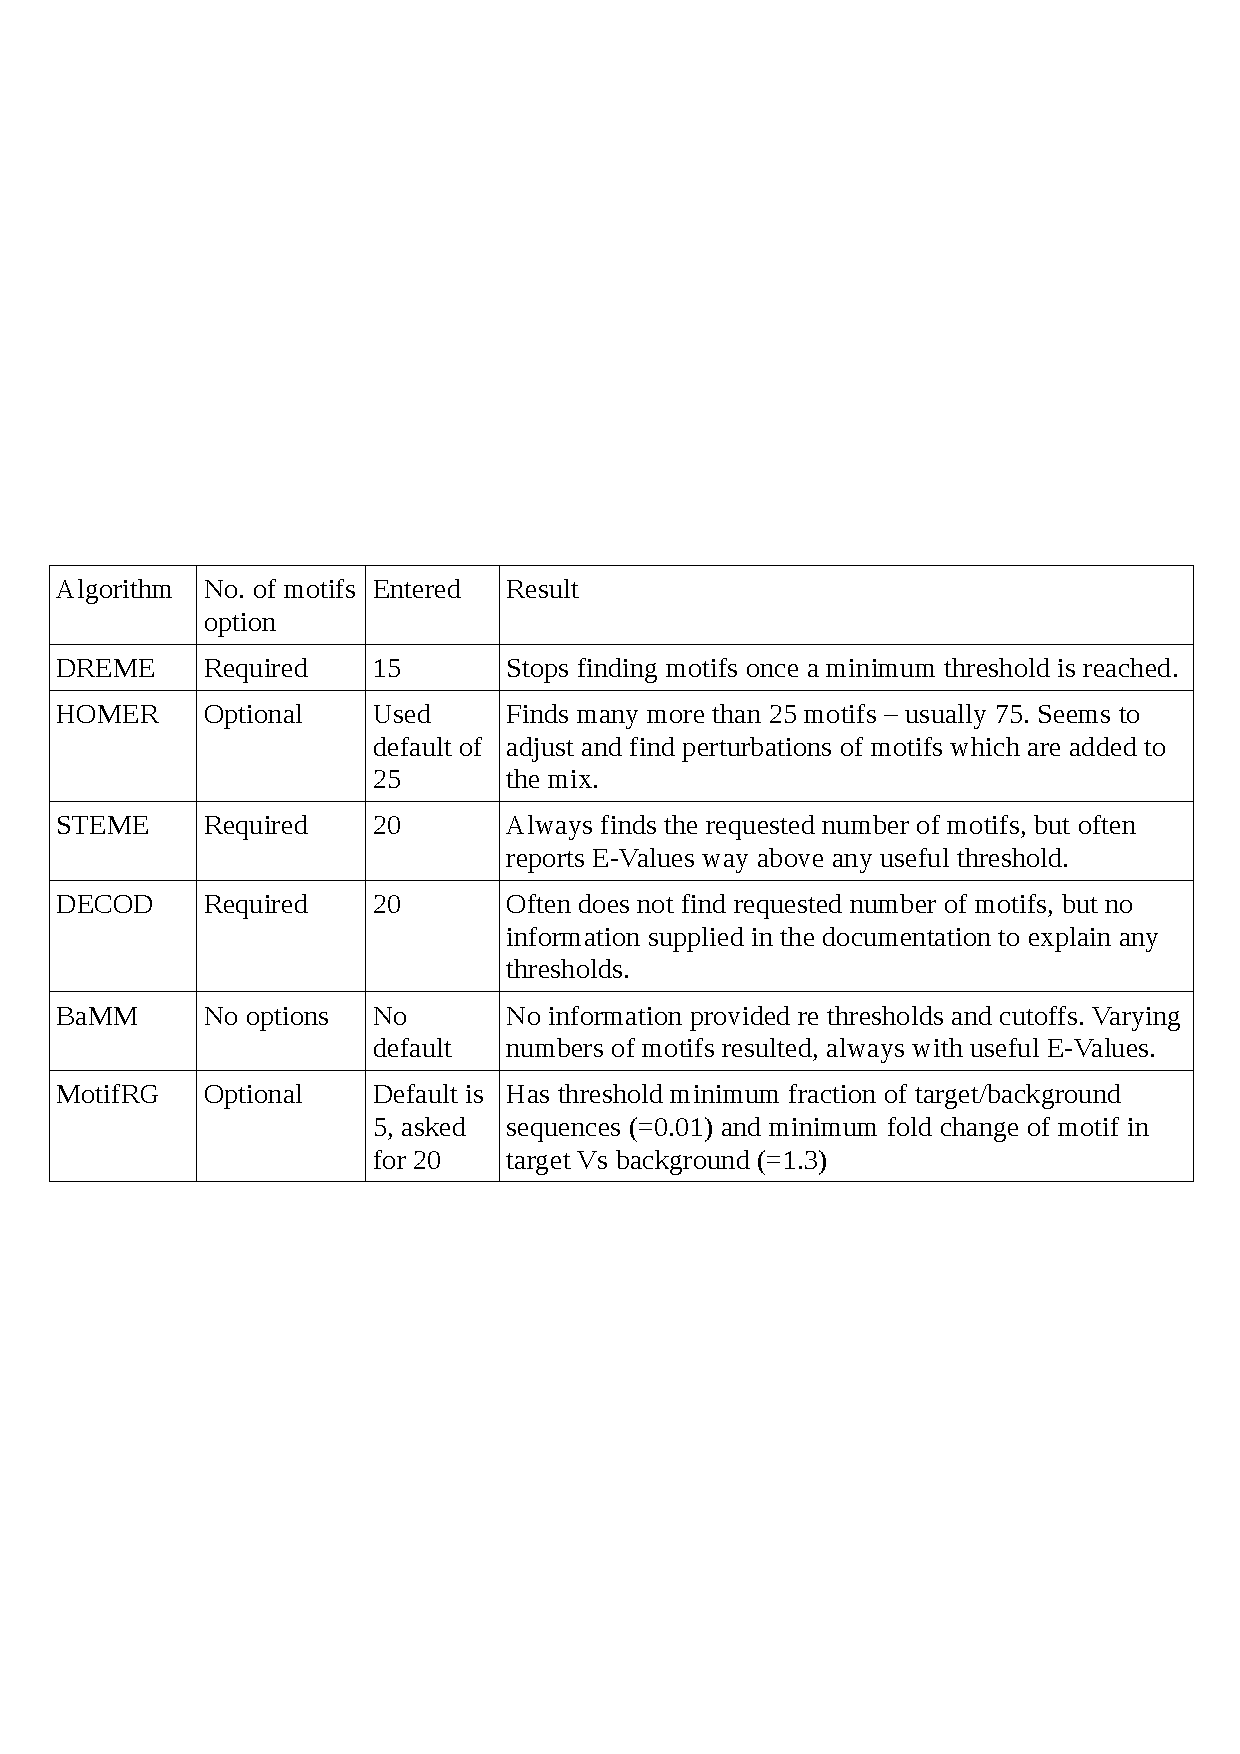
\includegraphics[width= \textwidth]{plots/algorithm_summary.pdf} 
    \caption{{\bf Summary of motif detection algorithm properties.}}
    \label{fig: motif_summary}
\end{table}

\subsection{Results from pilot study}

The six different algorithms returned a total of 770 motifs in the exon sequences, illustrated in the circular cladogram developed using Evolview tree viewing software  \citep{he2016evolview}. Although the number of motifs means that the labelling on the cladogram is not easily distinguishable, the colouring provides an 
illustration of the number and spread of motifs found by each algorithm. In the exon sequences, HOMER found the most motifs, with good variability, with 
each set of motifs possibly representing a unique transcription factor binding site. BaMM!motif and STEME both have a similar spread to HOMER, without the sets of motifs for each hierarchical 
branch. A total of 770 motifs were detected in the exon sequences with all the motifs identified as potential binding sites for transcription factors. 
Table 4 shows the TF motif E74A with 38 motifs matching.

\begin{figure}[ht] 
     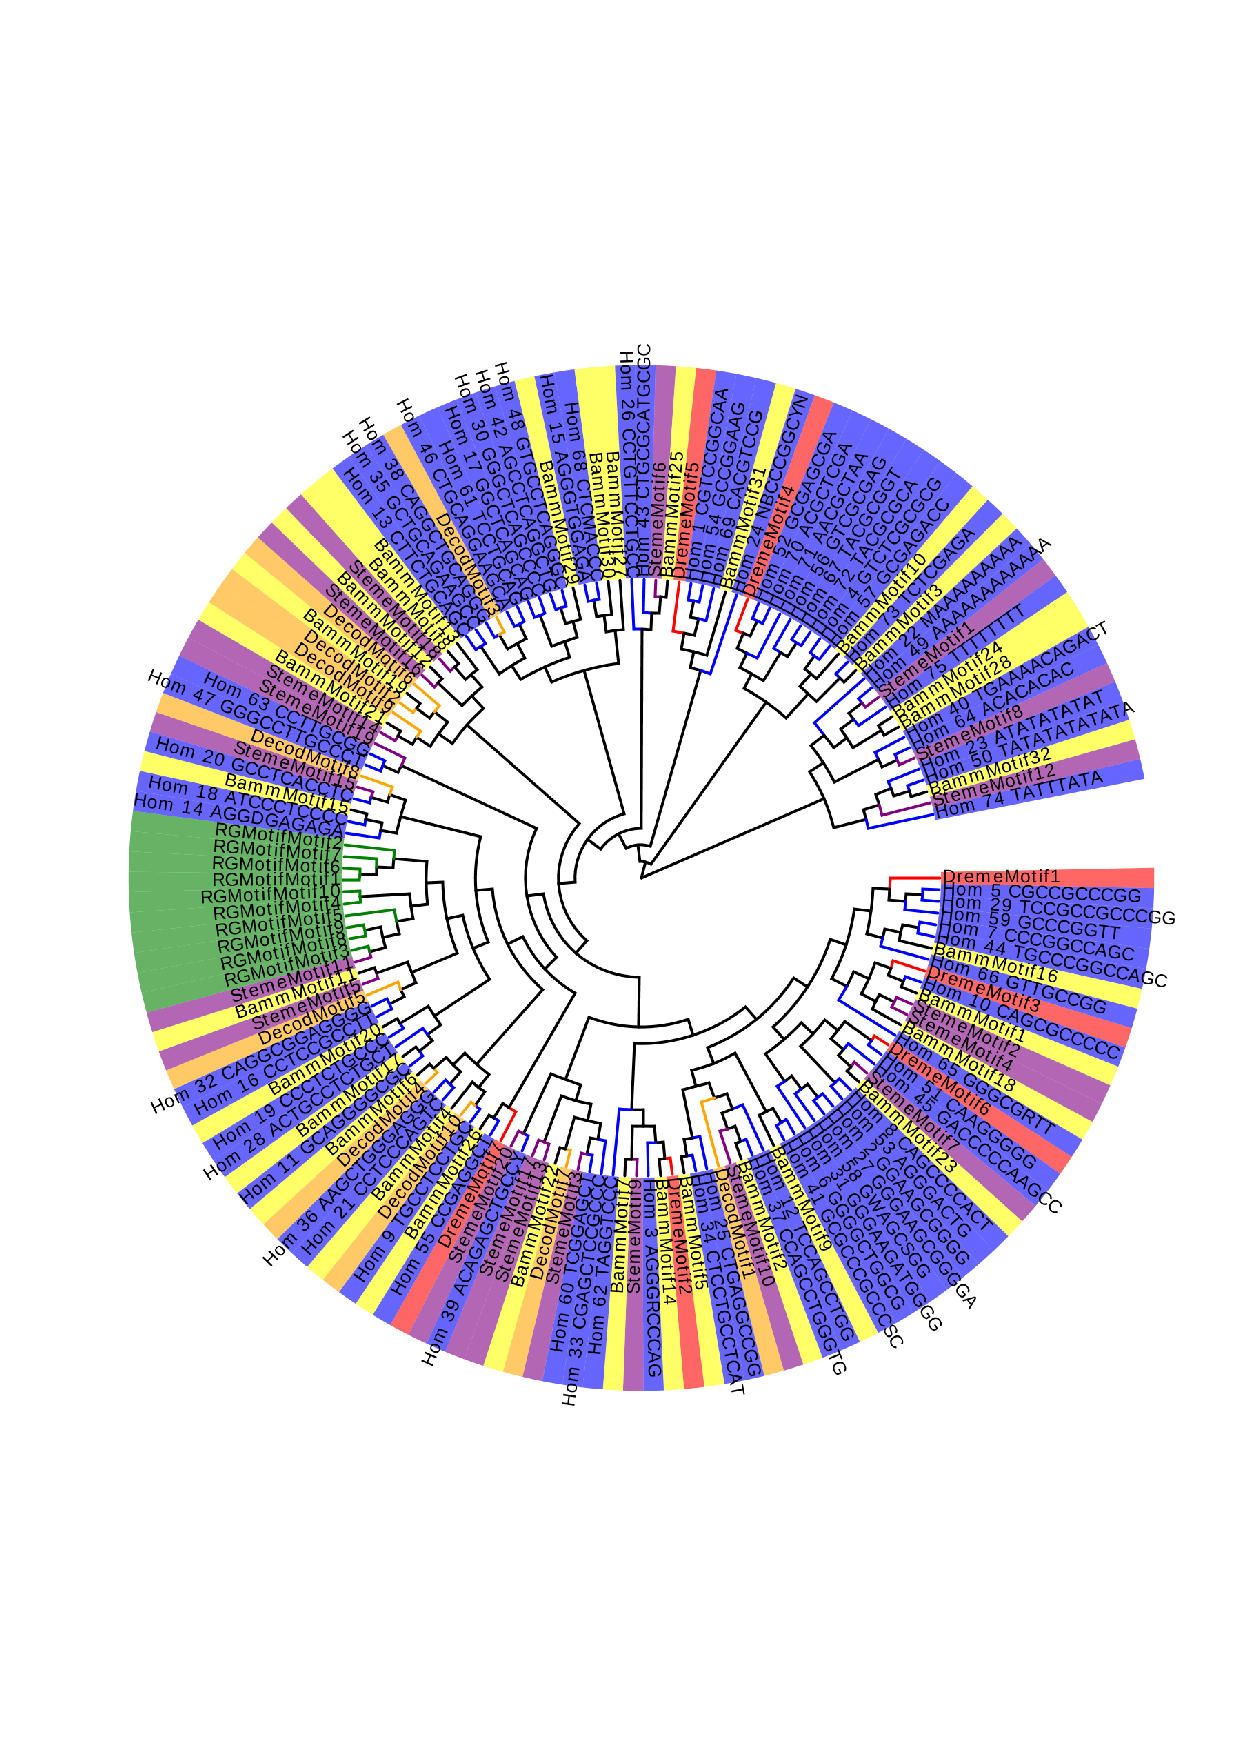
\includegraphics[width= \textwidth]{plots/exon_pilot_cardiogram.pdf} 
    \caption{{\bf Circular cladogram of 770 exon motifs from Evolview tree viewing software \cite{he2016evolview} }. 
    The cladogram depicts motifs detected from DREME (red), HOMER (blue), BaMM (yellow), MotifRG (green), STEME (purple)
    and DECOD (orange). }
    \label{fig: exon_cladogram}
\end{figure}

All of the motifs were identified as potential binding sites for transcription factors \textcolor{red}{Using the STAMP algorithm?}. It is often the case that a single transcription factor has many binding sites. For this reason the 770 motifs were identified as binding sites for 99 transcription factors, with more than half the motifs identified as potential binding sites for a subset of just 17 transcription factors, as illustrated in Table \ref{fig: motif_tf_summary_exons}. Similar results 
to the exon sequences were generated for intron, intergenic and promoter sequences.

We do not wish to delve too deeply in these results as they are the pilot results and are a guide. They show is that the algorithm are capable of detecting
motifs and allow us to discriminate between which algorithms may be best suited to the larger scale analysis.

\begin{table}[!h]
    \centering
     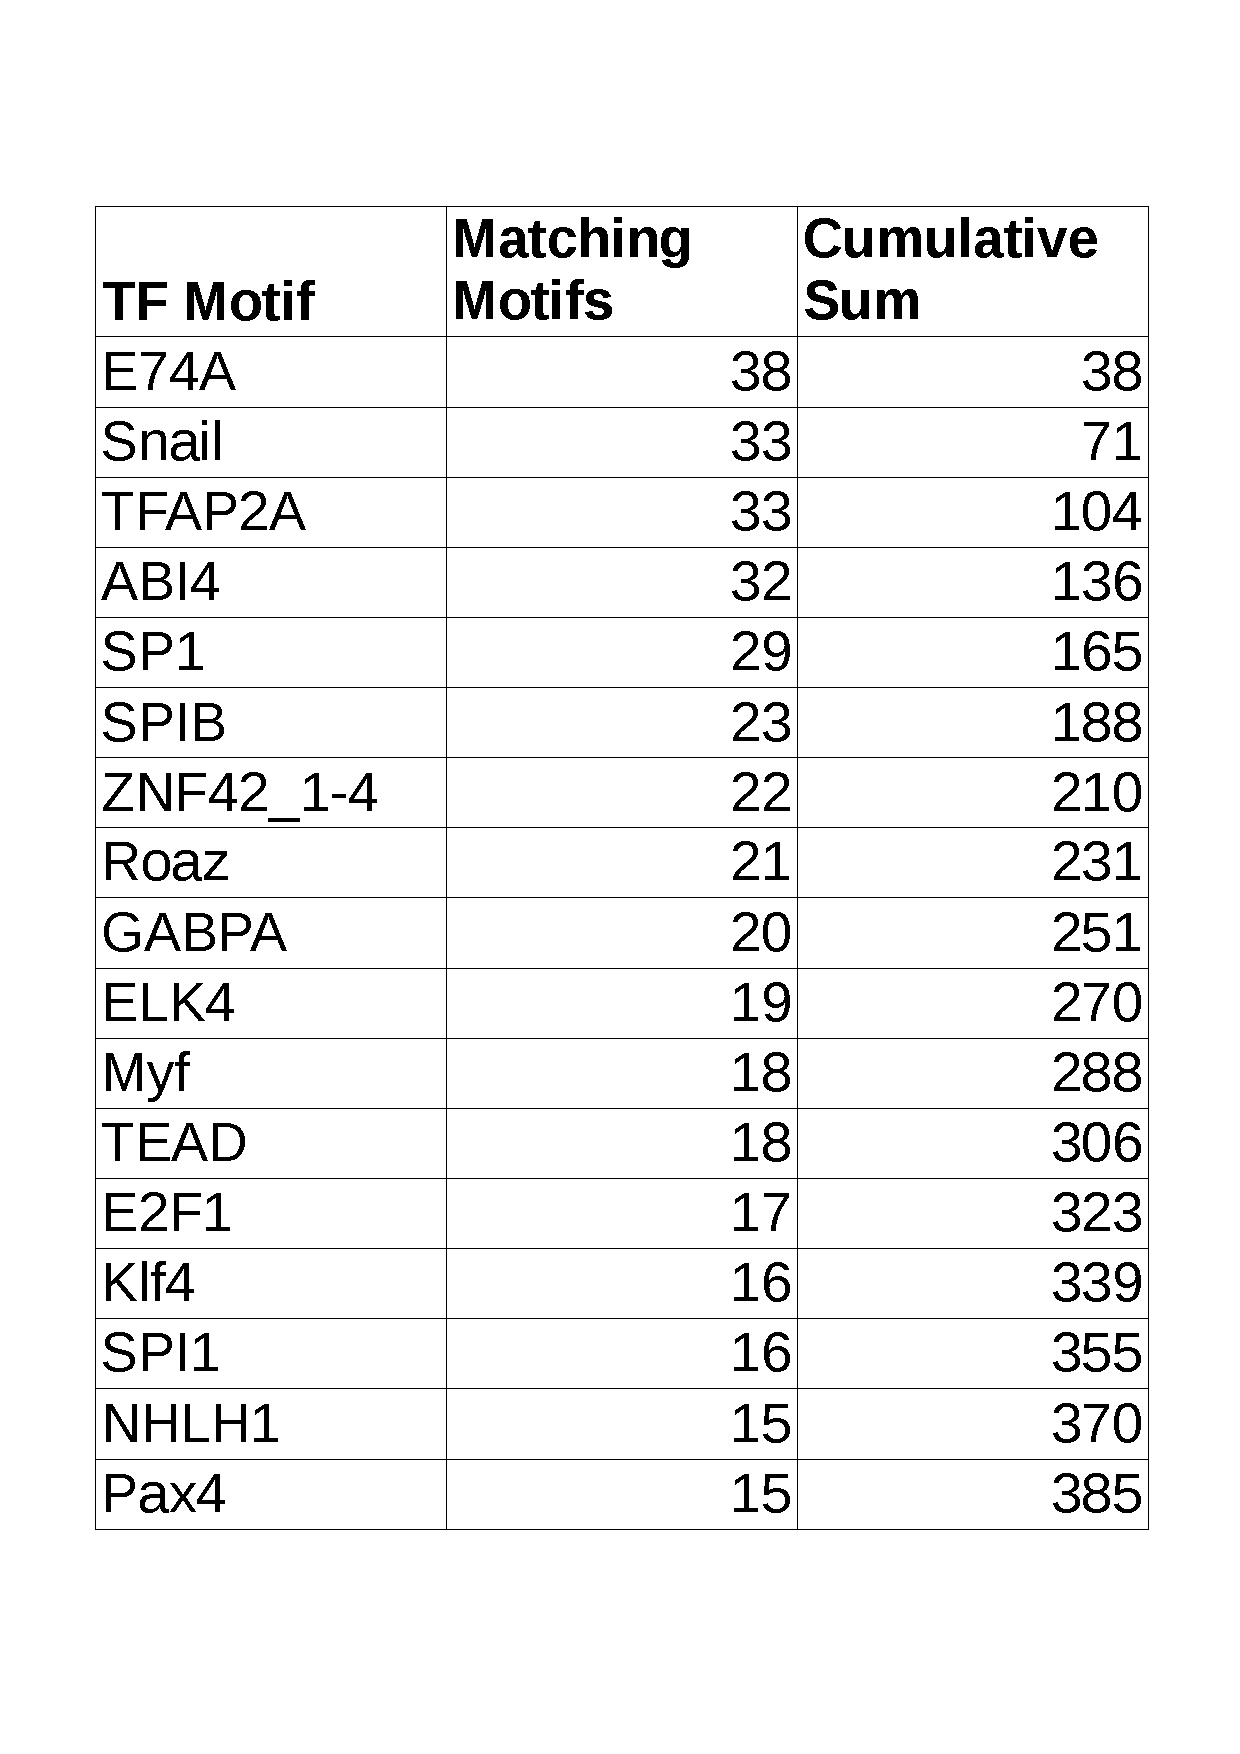
\includegraphics[width= 0.5\textwidth]{plots/table4_study.pdf} 
    \caption{{\bf Summary of transcription factor (TF) matches to motifs detected in exonic sequences in the pilot study.}}
    \label{fig: motif_tf_summary_exons}
\end{table}


The pilot study suggests that the two algorithms HOMER and BaMM!motif appear to have the most extensive coverage of motif binding sites. The recently published BaMM!motif algorithm is particularly impressive, given the fine tuning of its motifs, unlike HOMER, whose motifs are frequently clumped into broad clusters. Both these motif finding algorithms have high computational efficiency making them well suited to the large sequence analysis. DREME is also 
efficient, but fails to find some motifs that are found by every other algorithm. This is also the case for DECOD, which is computationally inefficient. STEME is
likewise very inefficient, and reports E-Values at odds with those reported by the other algorithms. Finally, motifRG seems to miss many motifs and fails to report the significance of those it finds. Therefore, for the larger scale analysis we will attempt to just use HOMER and BaMM!motif.

\begin{table}[!h]
    \centering
     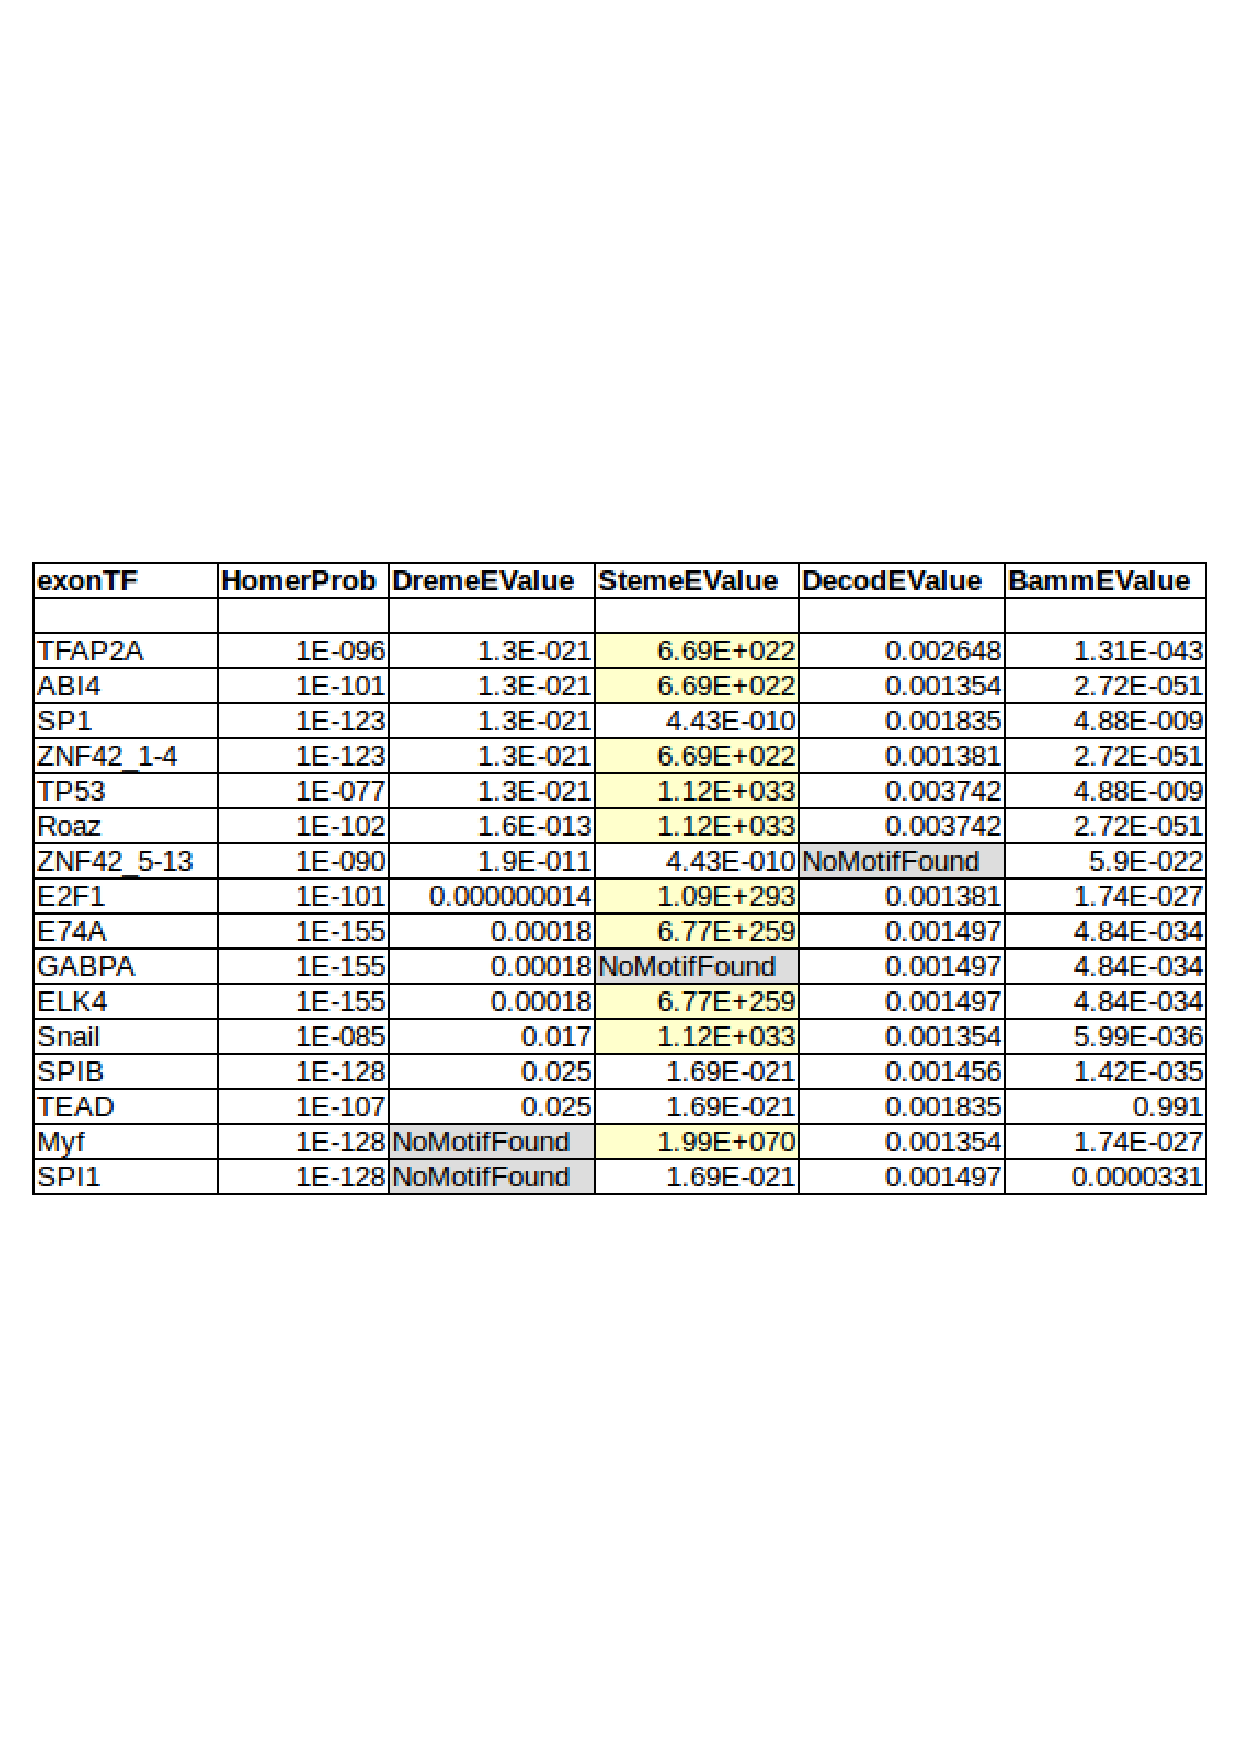
\includegraphics[width= \textwidth]{plots/exon_common.pdf} 
    \caption{{\bf TFs found by all algorithms with associated E-Values, ordered by DREME E-Values in pilot exon sequences.}}
    \label{fig: motif_tf_summary_exons}
\end{table}

\clearpage
\subsection{Moving from 200 kb sequences to larger sequences}

The pilot data looked at small regions surrounding the eQTLs. The full analysis will look at much longer sequences, which could dramatically increase
the computational challenge relative to the pilot study.  Sequences of four different lengths: 200001 bases; 40001 bases; 10001 bases; and 2001 bases) (termed 200KB, 40KB, 10KB and 2KB sequences) were created, all centred on the eQTLs listed used in the pilot study. The same length sequences were also created 
for the variants with no effect (termed null sequences). The purpose of this investigation was to determine whether target sequences might overlap with null sequences. The likelihood of overlap increases with the length of the sequence. Substantial overlap reduces the ability of algorithms to discriminate between target and null sequences when searching for relative motif enrichment. A python program was written to isolate all overlaps. If an eQTL sequence had more than one overlap (e.g. with different null sequences overlapping the start and finish of the eQTL sequence), the largest overlap was used to calculate the size of the overlap. An R program was used to convert these overlaps into a histogram of the number of overlapping sequences as a percentage of all sequences within each chromosome.

Figure \ref{fig: 100kbOverlaps}(a) provides a histogram of the percentage of eQTL sequences that overlapped with null sequences by chromosome for the 200 kb sequences. As illustrated, a majority of chromosomes had at least 40 percent of their sequences with some degree of overlap, with close to 80 percent of sequences in three chromosomes overlapping with null sequences. Twenty percent of sequences in almost every chromosome fell into this category, and for chromosome 13, sixty percent of sequences had at least 50 percent overlap  \ref{fig: 100kbOverlaps}(a).


%\begin{table}[!h]
%    \centering
%     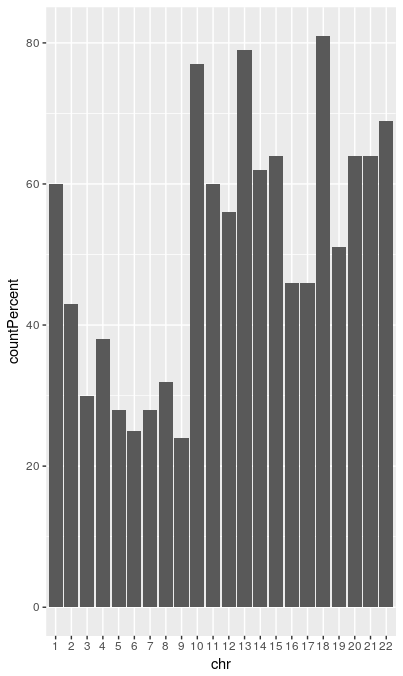
\includegraphics[width= 0.5\textwidth]{plots/100kbOverlapCount.png} 
%    \caption{{\bf Summary of percentage of eQTL and null sequences that overlap for 200 kb sequences.}}
%    \label{fig: 100kbOverlaps}
%\end{table}

\begin{figure}[!htbp]%
\centering
\subfloat[All 200 kb sequences with overlap]{{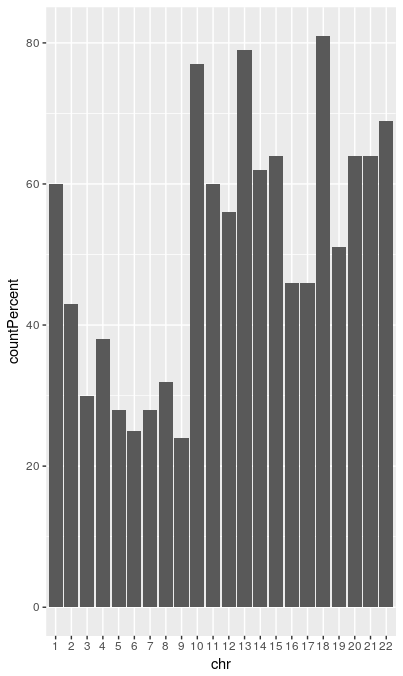
\includegraphics[height=10cm]{plots/100kbOverlapCount.png} }}%
\qquad
\subfloat[200 kb sequences with 50 percent overlap]{{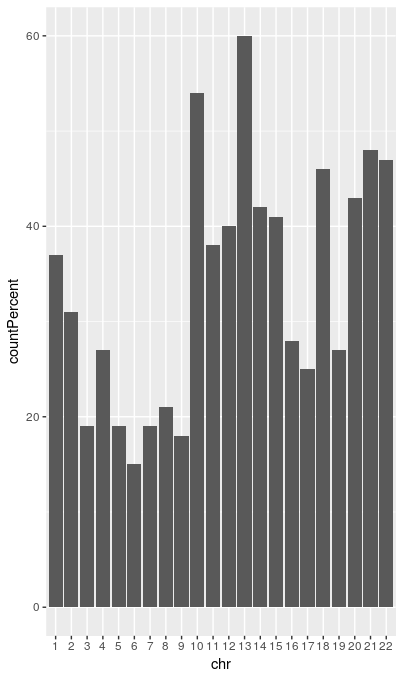
\includegraphics[height=10cm]{plots/100kbSequencesWith50PercentOverlap.png} }}% 
\caption{Summary of overlap percentage of eQTL and null sequences for 200 kb sequences with overlaps}
\label{fig: 100kbOverlaps} 
\end{figure}  


For 40KB sequences, the percentage of eQTL sequences that overlapped with null sequences by chromosome, with no account taken on the size of the overlap 
was approximately 20\%. Only one chromosome had more than 30 percent of sequences overlapping with null sequences, although all chromosomes had at least ten percent of their sequences with some overlap. Only one chromosome had more than 15 percent of its sequences with 50 percent overlap or more. For 10 kb sequences, the overlap is substantially reduced. A maximum of eight percent of sequences in any chromosome experience any overlap with on average 
four percent of the sequences having overlap greater than 25\% on average across the genome.

Finally, Figure \ref{2kbOverlaps} illustrates the amount of overlap when sequence length is restricted to 1000 bases on either side of the variant (2 kb sequences). Figure \ref{2kbOverlaps}(a) shows the percentage of all overlaps within each chromosome, and Figure \ref{2kbOverlaps}(b) shows the percentage of sequences that overlap by at least 25 percent. As shown in this figure, almost all chromosomes have only 1 or 2 percent overlapping sequences, and only 1 or 2 percent overlap by more than 25 percent.

\begin{figure}[!htbp]%  
\centering
\subfloat[All 2 kb sequences with overlap]{{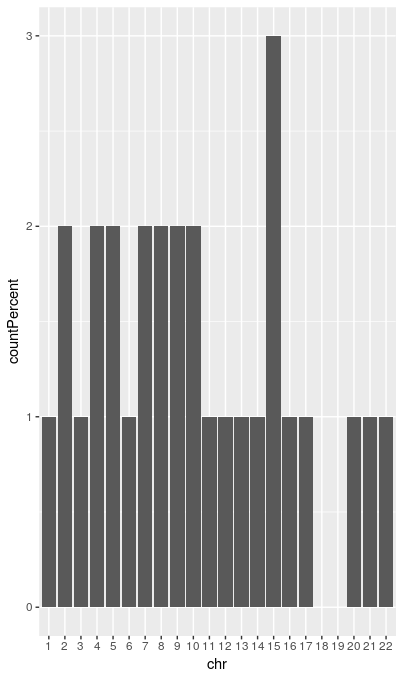
\includegraphics[height=10cm]{plots/1kbSequencesOverlap.png} }}% 
\qquad
\subfloat[2 kb sequences with 25 percent overlap]	{{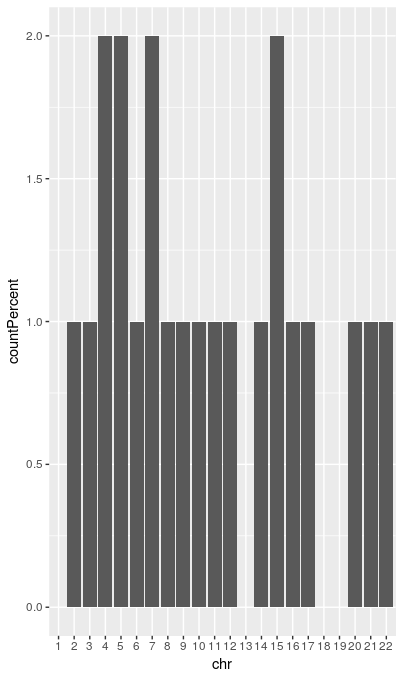
\includegraphics[height=10cm]{plots/1kbSequences25PercentOverlap.png} }}% 
\caption{2 kb sequence overlap between null and eQTL sequences.}\label{2kbOverlaps}%
\end{figure}  

This analysis indicates that a using sequences of length 2001 base pairs is a good compromise between computational efficiency and minimising sample
overlap.
 

\section{Large scale motif detection analysis of 2 kb sequences}

Propose to use HOMER  \citep{heinz2010simple} and BaMM!motif algorithms \citep{siebert2016bayesian} to analyse genomic sequence centred at 
the eQTL discovered in \citet{lloyd2017genetic}. The null sequences will be generated as per the pilot study with 2 kb sequences around null variants from
the \citet{lloyd2017genetic} gene expression study.

\subsection{Detailed description of application of HOMER and  BaMM!motif algorithms}

\begin{itemize}
\item How were the sequences generated
\item How were the sequences encoded into a format for use with the algorithms
\item What defaults/parameters were used when running each of the algorithms
\item What sort of computer was used to run the analyses and what were their run times
\end{itemize}

\subsection{Detailed description of null versus null sequence validation}

This analysis was motivated by the want to have a gauge of whether these algorithms will detect motifs in sets of
sequences that should be similar i.e., they may contain motifs but they should not be enriched in the target versus
background sequences.

\begin{itemize}
\item Original was the null versus scrambled null sequences. 
\item Better to do half vs other half for the null sequences.
\end{itemize}

\subsection{Detailed description of HOMER and  BaMM!motif output}

This will form the main component of your report.

\begin{itemize}
\item For each of the algorithms there is an evaluation of the enrichment of a motif in the target versus background sequences. What tests are used to
evaluate the evidence for enrichment for each of these algorithms? 
\item What other output is generated from each algorithm. The actual motifs? Description of an substitution bases like $N$ or $Y$ in the motifs. Do the
algorithms tell you where the motifs were in the target sequences? Do they tell you how many motifs were in the target versus background sequences.
Do they program manuals give you any heuristics for deciding that a motif is genuinely a motif?
\end{itemize}

\subsection{Potential confounders}

Maybe the null sequences are not so null?

\begin{itemize}
\item We could compare the eQTL sequences and null sequences to make sure they are relatively balanced for LD content, MAF. Mention that HOMER controls for GC content. 
\end{itemize}

\subsection{Results}

\begin{itemize}
\item How many motifs were detected in total for each algorithm in the eQTL vs null sequences and then the null versus null analysis?
\item How many were robustly associated i.e., passing the corrected significance threshold for each algorithm. Hopefully some for the eQTL versus background
and none or very few uninteresting ones for the null versus null.
\item We need to think about how we validate these. Initial investigation with STAMP. Look up in ECODE UCSC
\end{itemize}


\subsection{Discussion}

\begin{itemize}
\item Reflect on the initial aim of the study
\item What have we learnt
\item What can we conclude
\item More to come
\end{itemize}




\clearpage
\section{Miscellaneous}

The TATAAT box is a well conserved sequence centered around 10 bp upstream of transcription initiation. This motif forms the binding site for a subunit of
the RNA polymerase. Despite the high degree of conservation it extremely rare to find a promoter that matches this consensus exactly. The activity of the
promoter is related to how well it matches the consensus sequence and so the activity of each gene can be fine tuned by how much its region deviates from
the consensus. The affinity of a DNA binding site is typically correlated wit how well the site matches the consensus sequence. Not all positions in a binding
site are equally forgiving of mismatches and not all mismatches have the same effect \citet{d2006dna}.

Promoters initiate transcription. Studies of eQTL in human and model systems have identified functional genetic variants in the vicinity of promoters that affect transcript abundance \citet{schor2017promoter}. There exist narrow promoters and broad promoters are present in mammalian genomes and form
the basis of the phenotype promoter shape. Broad promoters have more dispersed patterns of transcriptional initiation and do not contain a TATA box. 

Deciphering the DNA sequences bound by TFs is critical for elucidating transcriptional regulation of gene expression. 

\citet{linhart2008transcription}  states that one of the main cellular mechanisms is the transcriptional program, which describes when and to what etent each gene is transcribed to mRNA. Transcription is primarily driven by transcription factors, which bind sequence elements primarily in a gene's promoter sequence upstream from the transcription start site. Another key regulatory effect is controlled by microRNAs short non-coding RNA molecules. Annealing of the microRNA to the target nRNA triggers the degradation of the mRNA transcript or inhibits protein translation. 

The classical way to identify motifs is by identifying recurring sequence patterns in cis-regulatory sequences. Given a target set of co-regulated genes
one would like to identify motifs that statistically overrepresented in the promoters of these genes, compared with some background model or with a 
supplied reference set of genes.   

The enrichment scores used in the motif detection algorithms might fail if the distribution of the length of GC content of the target sequences significantly
differs from the background set. There is also a length bias in 3' UTR of tissue specific genes. \citet{linhart2008transcription} overcome this by putting genes
in bins of similar length and GC content. 

Comparison of discovered motifs with a database of known motifs is done quite often within this field. The use of STEME then seems quite natural. 

\clearpage
\bibliographystyle{plainnat}
\bibliography{bibtexfile}
























\end{document}

